\chapter{Reprodução sexuada dos mamíferos}\label{ch:b2:mammal-reproduction}

Um óvulo humano tem um décimo de milímetro de diâmetro e é a maior
célula do corpo; um espermatozoide é um núcleo com uma hélice, um entre
trezentos milhões liberados de uma só vez, dos quais algumas dezenas
chegarão ao óvulo e um só entrará nele. Em uma semana, o óvulo
fecundado se tornou uma esfera oca que se aprofunda na parede do útero
e constrói, a partir de suas próprias células externas, um órgão --- a
\omterm{def:b2:mammal-reproduction:placenta}{placenta} --- através do qual a mãe o alimentará durante nove meses.
Depois ele nasce e é alimentado com leite. Todo mamífero faz isso;
nenhum outro animal faz tudo isso. Este capítulo acompanha os gametas
até a fecundação, o embrião até a \omterm{def:b2:mammal-reproduction:implantation}{implantação} e o organismo ao longo da
gestação, do parto e da lactação, e termina com o modo como os dois
sexos são formados.

\section{Gônadas e gametas}

\begin{definition}[O testículo e a espermatogênese]\label{def:b2:mammal-reproduction:testis}
\index{espermatogênese}\index{túbulo seminífero}\index{célula de Sertoli}\index{célula de Leydig}
O \emph{testículo} é uma massa de \emph{túbulos seminíferos}, com
várias centenas de metros no total, cujas paredes produzem os
espermatozoides; entre os túbulos ficam as \emph{células de Leydig},
que produzem testosterona. Na parede do túbulo, as
\emph{espermatogônias} da borda externa se dividem por mitose,
mantendo uma população de células-tronco e enviando células para o
interior; estas crescem em \emph{espermatócitos} primários, que passam
pela \omterm{def:b2:meiosis-heredity:meiosis}{meiose} I (dando dois espermatócitos secundários) e pela \omterm{def:b2:meiosis-heredity:meiosis}{meiose} II
(dando quatro \emph{espermátides} \omterm{def:b2:meiosis-heredity:meiosis}{haploides}); as espermátides perdem a
maior parte do citoplasma, condensam o núcleo, desenvolvem um flagelo
e cobrem o núcleo com o \emph{acrossomo}, uma vesícula de enzimas,
tornando-se \emph{espermatozoides}, que são liberados na luz do túbulo.
Grandes \emph{células de Sertoli} atravessam a parede, nutrem as
células germinativas e formam, por junções oclusivas entre si, uma
\emph{barreira hematotesticular} que mantém o sistema imune afastado
de células que só aparecem na puberdade. A sequência inteira leva
cerca de \num{64} dias no homem e produz uns $10^{8}$ espermatozoides
por dia, da puberdade à velhice. Os espermatozoides saem do testículo
imóveis e amadurecem no \emph{epidídimo} durante duas semanas.
\end{definition}

\begin{omfigure}
\begin{tikzpicture}[every node/.style={font=\scriptsize}]
  % tubule cross-section: concentric layers
  \draw[thick, fill=omExo!15] (0,0) circle (2.5);
  \draw[thick, fill=omExo!8] (0,0) circle (2.2);
  \draw[thick, fill=omDef!10] (0,0) circle (1.6);
  \draw[thick, fill=omProp!12] (0,0) circle (1.0);
  \draw[thick, fill=white] (0,0) circle (0.45);
  % cells
  \foreach \a in {0,30,...,330} \draw[thick, fill=omDef!40] (\a:2.0) circle (0.13);
  \foreach \a in {15,45,...,345} \draw[thick, fill=omDef!70] (\a:1.32) circle (0.16);
  \foreach \a in {0,20,...,340} \draw[thick, fill=omProp!60] (\a:0.75) circle (0.08);
  \foreach \a in {10,40,...,340} \draw[thick, omProp!80!black] (\a:0.45) -- (\a:0.15);
  % Sertoli cell: tall wedge
  \draw[thick, omExo!70!black, fill=omExo!40, opacity=0.6] (100:2.2) .. controls (90:1.6) and (95:0.9) .. (92:0.5) .. controls (80:0.9) and (75:1.6) .. (72:2.2) -- cycle;
  % Leydig cells outside
  \foreach \p in {(2.9,0.8),(3.1,0.3),(2.8,-0.3)} \draw[thick, fill=omThm!40] \p circle (0.14);
  % labels
  \draw (2.0,0) -- (3.6,-0.5) node[right, align=left] {espermatogônias ($2n$)\\na borda externa};
  \draw (1.32,-0.7) -- (3.6,-1.5) node[right, align=left] {espermatócitos primários\\(meiose I)};
  \draw (0.75,-0.4) -- (3.6,-2.4) node[right, align=left] {espermátides ($n$)};
  \draw (0.3,-0.2) -- (3.6,-3.1) node[right, align=left] {espermatozoides na luz};
  \draw (2.95,0.55) -- (3.6,0.6) node[right, align=left] {células de Leydig:\\testosterona};
  \draw (88:1.4) -- (3.6,1.8) node[right, align=left] {célula de Sertoli atravessando a parede};
  \node[anchor=east, align=right] at (-2.7,0) {exterior\\(lâmina basal)};
\end{tikzpicture}

{\small Um \omterm{def:b2:mammal-reproduction:testis}{túbulo seminífero} em corte transversal. As células
germinativas amadurecem da parede externa (espermatogônias) para o
interior (espermatócitos, espermátides, espermatozoides na luz),
sustentadas pelas \omterm{def:b2:mammal-reproduction:testis}{células de Sertoli}; as \omterm{def:b2:mammal-reproduction:testis}{células de Leydig}, entre os
túbulos, produzem testosterona.}
\end{omfigure}

\begin{omfigure}
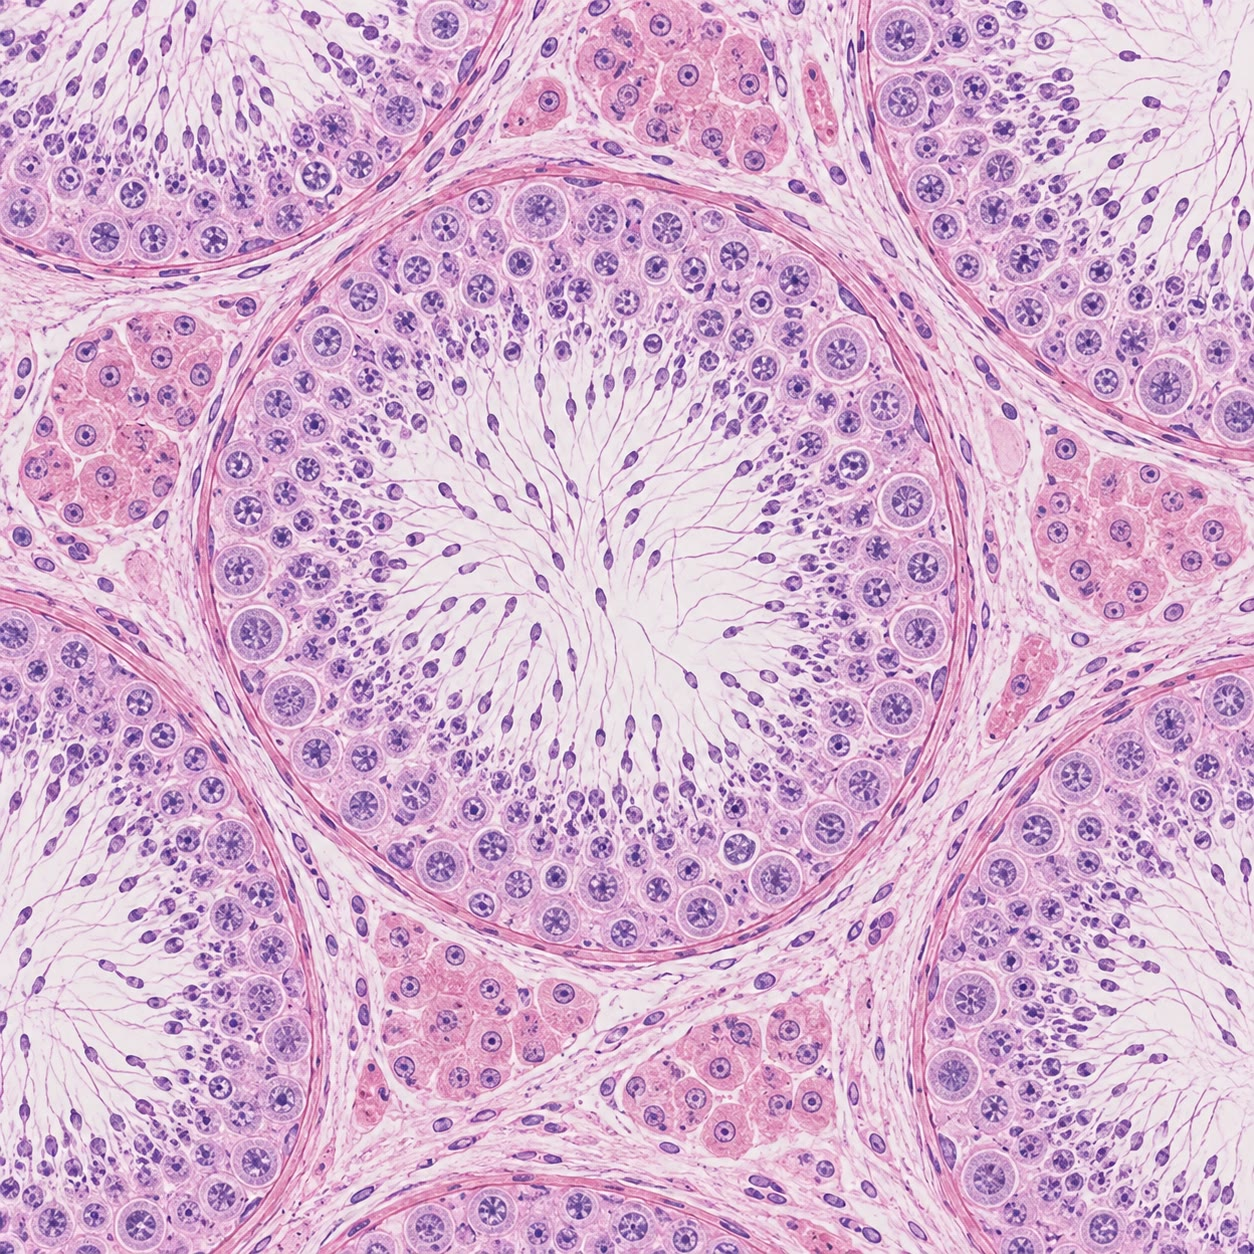
\includegraphics[width=0.42\linewidth]{images/book4/ai/b4-08-testis-histology.jpg}\hspace{0.04\linewidth}
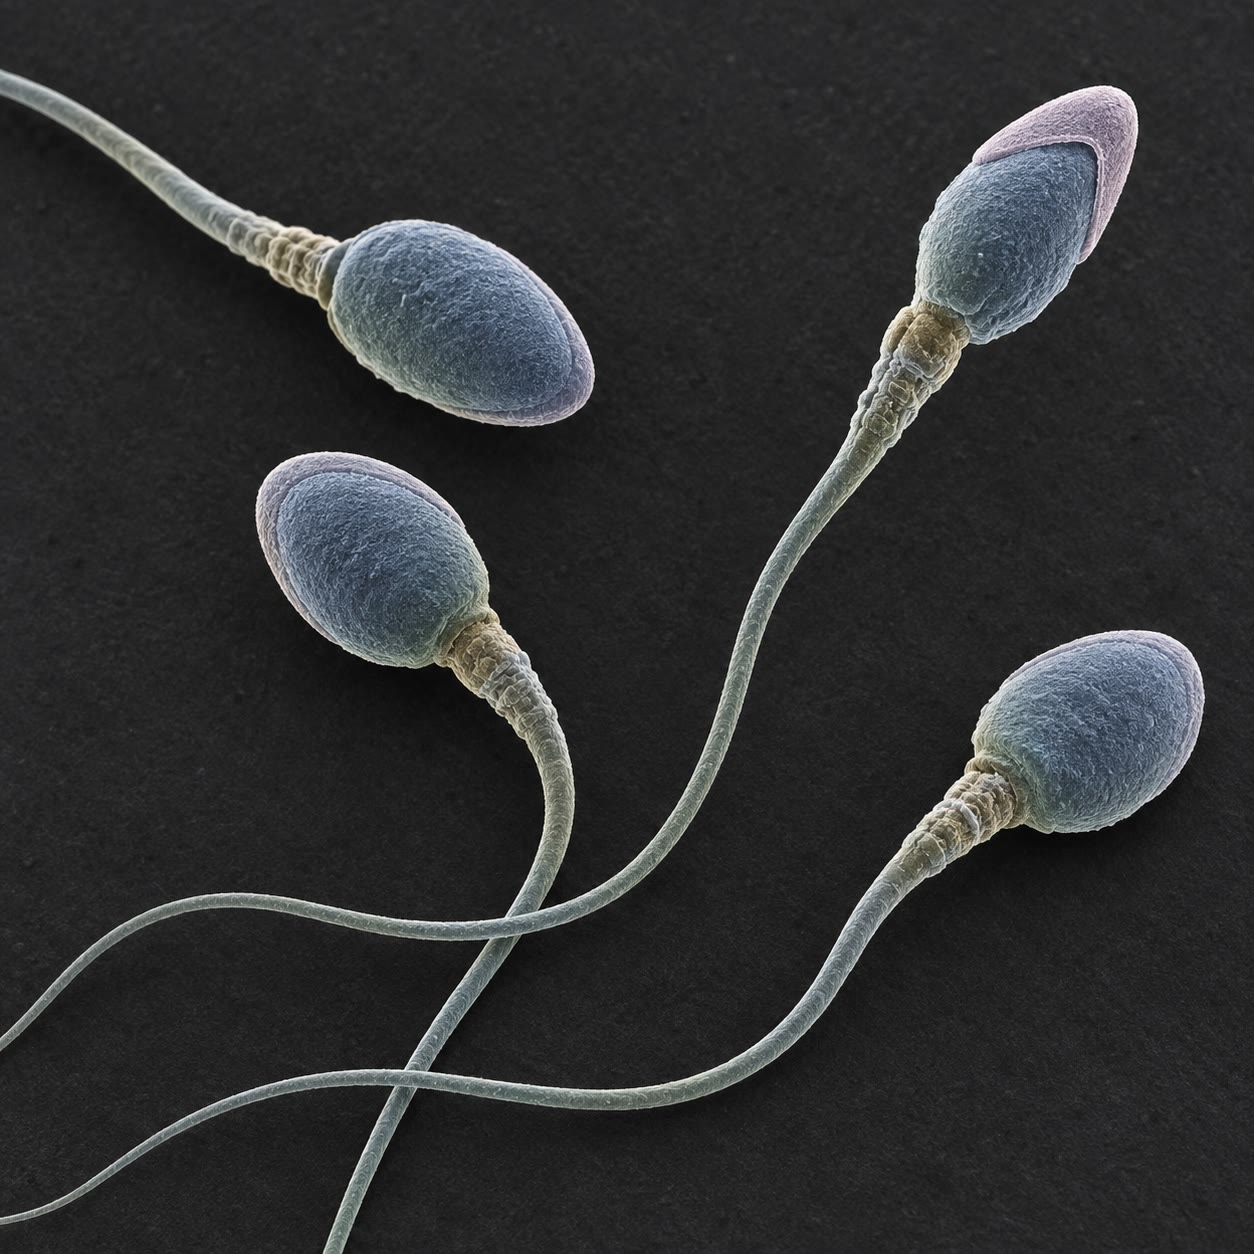
\includegraphics[width=0.42\linewidth]{images/book4/ai/b4-08-sperm-sem.jpg}

{\small À esquerda: \omterm{def:b2:mammal-reproduction:testis}{túbulos seminíferos} em corte, com as células
germinativas dispostas em camadas da parede até a luz. À direita:
espermatozoides ao microscópio eletrônico de varredura, com o capuz
acrossômico visível nas cabeças.}
\end{omfigure}

\begin{definition}[O ovário e a ovogênese]\label{def:b2:mammal-reproduction:ovary}
\index{ovogênese}\index{folículo}\index{ovulação}\index{corpo lúteo}
A ovogênese é a imagem espelhada da \omterm{def:b2:mammal-reproduction:testis}{espermatogênese} em quase todos os
aspectos. As \emph{ovogônias} só se multiplicam no feto: ao nascer, uma
menina tem um estoque de cerca de um milhão de \emph{ovócitos}
primários, cada um parado na \omterm{prop:b2:meiosis-heredity:stages}{prófase I} da \omterm{def:b2:meiosis-heredity:meiosis}{meiose} e envolto por uma
única camada de células --- um \emph{folículo primordial} ---, e nenhum
novo jamais é produzido. A partir da puberdade, a cada mês uma coorte
de folículos cresce: o ovócito aumenta, as células da
\emph{granulosa} que o cercam se multiplicam em camadas, forma-se uma
\emph{teca} externa, abre-se uma cavidade cheia de líquido (o
\emph{folículo de Graaf}, com dois centímetros de diâmetro) e, em
geral, um único folículo chega à \emph{ovulação}: o ovócito, que só
agora completa a \omterm{def:b2:meiosis-heredity:meiosis}{meiose} I e para de novo na metáfase II, é expulso com
seu halo de células da granulosa para a tuba uterina. O folículo
esvaziado se torna o \emph{corpo lúteo}, uma glândula temporária de
progesterona. A \omterm{def:b2:meiosis-heredity:meiosis}{meiose} produz um óvulo e três minúsculos corpúsculos
polares --- todo o citoplasma vai para uma célula ---, e a \omterm{def:b2:meiosis-heredity:meiosis}{meiose} II só
se completa se um espermatozoide entrar. Do milhão de ovócitos, cerca
de \num{400} são ovulados ao longo da vida; os demais degeneram
(\emph{atresia}) e, quando o estoque se esgota, por volta dos cinquenta
anos, os ciclos param: é a menopausa.
\end{definition}

\begin{omfigure}
\begin{tikzpicture}[every node/.style={font=\scriptsize}, >=stealth]
  % timeline of oogenesis vs spermatogenesis
  \draw[thick, ->] (0,3.0) -- (12.6,3.0); \node[anchor=west] at (12.6,3.0) {idade};
  \foreach \x/\l in {0/{feto}, 2.2/{nascimento}, 4.6/{puberdade}, 10.2/{$\sim$50 anos}}
    \draw (\x,3.1) -- (\x,2.9) node[above=0.15cm] {\l};
  % oogenesis line
  \node[anchor=east, omThm] at (-0.2,1.5) {ovogênese};
  \draw[very thick, omThm] (0,1.5) -- (1.6,1.5); \node[above, omThm, align=center] at (0.8,1.55) {ovogônias\\se multiplicam};
  \draw[very thick, omThm, dashed] (1.6,1.5) -- (4.6,1.5); \node[below, omThm] at (3.1,1.45) {parada na prófase I};
  \draw[very thick, omThm] (4.6,1.5) -- (10.2,1.5); \node[above, omThm, align=center] at (7.4,1.55) {uma ovulação por mês;\\meiose I completada na ovulação, II na fecundação};
  \fill[omThm] (10.2,1.5) circle (0.07); \node[below, omThm] at (10.2,1.45) {estoque esgotado};
  % spermatogenesis line
  \node[anchor=east, omDef] at (-0.2,0.3) {espermatogênese};
  \draw[very thick, omDef, dashed] (0,0.3) -- (4.6,0.3); \node[above, omDef] at (2.3,0.35) {espermatogônias quiescentes};
  \draw[very thick, omDef, ->] (4.6,0.3) -- (12.6,0.3); \node[above, omDef] at (8.6,0.35) {contínua: $10^{8}$ espermatozoides por dia, 64 dias cada, a partir de células-tronco};
\end{tikzpicture}

{\small As duas gametogêneses no tempo. Os ovócitos são todos
produzidos antes do nascimento e liberados um a um a partir de um
estoque finito; os espermatozoides são produzidos continuamente a
partir de células-tronco durante toda a vida adulta.}
\end{omfigure}

\begin{omfigure}
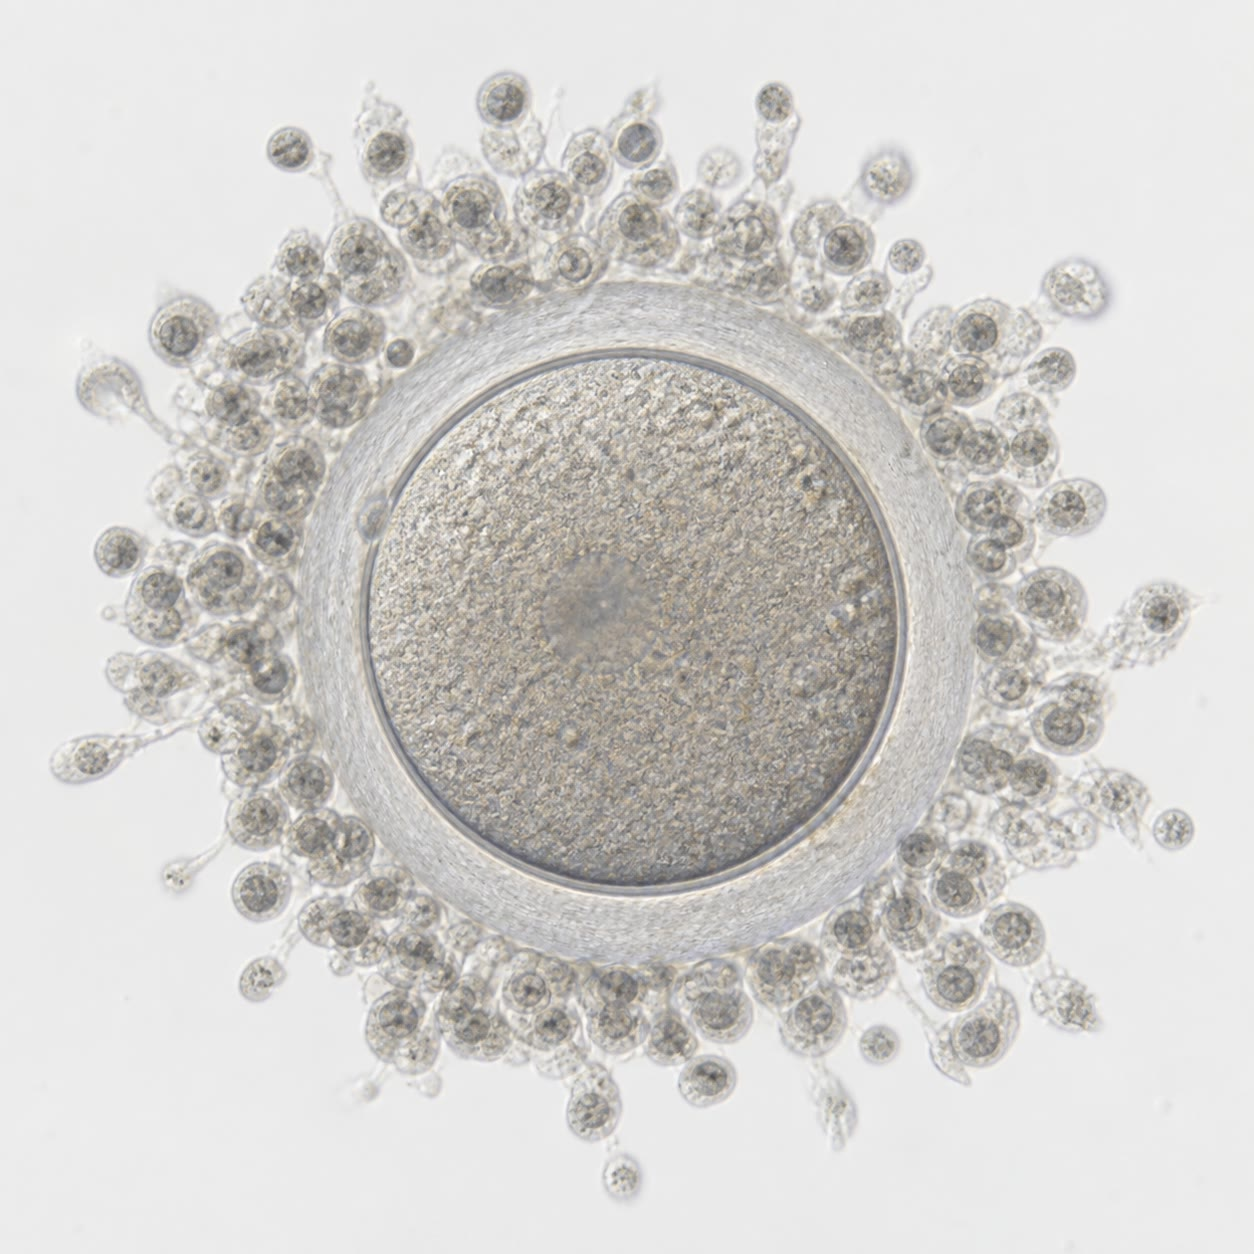
\includegraphics[width=0.46\linewidth]{images/book4/ai/b4-08-oocyte.jpg}

{\small Um ovócito ovulado: a célula, seu envoltório transparente (a
\omterm{prop:b2:mammal-reproduction:fertilisation}{zona pelúcida}) e a nuvem de células da granulosa que deixou o \omterm{def:b2:mammal-reproduction:ovary}{folículo}
com ela.}
\end{omfigure}

\section{A fecundação}

\begin{proposition}[As etapas da fecundação]\label{prop:b2:mammal-reproduction:fertilisation}
\index{fecundação!nos mamíferos}\index{reação acrossômica}\index{zona pelúcida}\index{reação cortical}
Os espermatozoides depositados na vagina --- cerca de $3\times 10^{8}$
--- atravessam o muco cervical, são levados útero acima por suas
contrações, e algumas centenas chegam em uma hora à ampola da tuba
uterina, onde o óvulo espera durante um dia. No caminho, os
espermatozoides passam pela \emph{capacitação}: secreções do trato
feminino removem proteínas de revestimento de suas membranas e os
tornam hiperativos. Junto ao óvulo, um espermatozoide atravessa as
células da granulosa, liga-se a uma glicoproteína da \emph{\omterm{prop:b2:mammal-reproduction:fertilisation}{zona
pelúcida}} e sofre a \emph{\omterm{prop:b2:mammal-reproduction:fertilisation}{reação acrossômica}}, liberando enzimas que
digerem um caminho através da zona; sua membrana se funde com a do
óvulo, e o núcleo do espermatozoide entra. O óvulo responde em
segundos: o cálcio se propaga por ele, e os grânulos corticais liberam
enzimas que endurecem a zona e removem seus receptores de
espermatozoides --- é a \emph{\omterm{prop:b2:mammal-reproduction:fertilisation}{reação cortical}}, o bloqueio da
polispermia. O óvulo completa a \omterm{def:b2:meiosis-heredity:meiosis}{meiose} II, expulsa o segundo corpúsculo
polar, e os dois \emph{pronúcleos} \omterm{def:b2:meiosis-heredity:meiosis}{haploides} replicam seu DNA, se
aproximam e entram na primeira mitose: o zigoto tem um dia. A
especificidade de espécie está nas proteínas da zona, e é por isso que
um espermatozoide de camundongo não entra num óvulo humano.
\end{proposition}
\begin{proof}[Evidências]
Edwards e Steptoe (1978) fecundaram um ovócito humano, retirado do
ovário pouco antes da \omterm{def:b2:mammal-reproduction:ovary}{ovulação}, com espermatozoides capacitados numa
placa, cultivaram o embrião até oito células e o devolveram ao útero,
onde ele se implantou e nasceu: a fecundação in vitro. Cada etapa da
sequência acima fora antes esclarecida no ouriço-do-mar e no
camundongo, em que a fusão, a onda de cálcio e a liberação dos grânulos
corticais podem ser observadas; no camundongo, a eliminação por
\omterm{def:b2:genome-diversification:mutation}{mutação} de uma glicoproteína da zona (ZP2 ou ZP3) produz óvulos aos
quais os espermatozoides não conseguem se ligar.
\end{proof}

\begin{theorem}[Por que um óvulo precisa de milhões de espermatozoides]\label{thm:b2:mammal-reproduction:poisson}
\index{polispermia}
Se, de $N$ espermatozoides depositados, cada um alcança a superfície
do óvulo de modo independente com uma pequena probabilidade $\pi$, o
número dos que chegam segue uma lei de Poisson de média $m = N\pi$, e a
probabilidade de que pelo menos um chegue é
\[
P = 1 - e^{-m}.
\]
Com $N = 3\times 10^{8}$ e $\pi \approx 10^{-8}$, $m \approx 3$
e $P \approx 0.95$; com $N = 2\times 10^{7}$ (o limiar clínico de
contagem baixa de espermatozoides), $m = 0.2$ e $P = 0.18$. A mesma
aritmética mostra por que o bloqueio da polispermia é indispensável:
quando $P$ é alto, vários espermatozoides chegam com poucos segundos de
diferença, e um óvulo penetrado por dois seria triploide e morreria.
\end{theorem}
\begin{proof}
Cada espermatozoide é uma tentativa independente, com probabilidade de
sucesso $\pi$; o número de sucessos é binomial, o que, para $N$ grande
e $\pi$ pequeno, dá uma lei de Poisson de média $N\pi$. A probabilidade
de zero sucessos é $e^{-m}$, logo a de pelo menos um é $1 - e^{-m}$; a
probabilidade de dois ou mais é $1 - e^{-m}(1 + m)$, cerca de $0.8$
para $m = 3$.
\end{proof}

\begin{omfigure}
\begin{tikzpicture}[every node/.style={font=\scriptsize}, >=stealth]
  \foreach \x/\lab in {0/{1. o espermatozoide\\se liga à zona}, 3.3/{2. reação acrossômica:\\enzimas abrem caminho}, 6.6/{3. fusão das membranas;\\onda de cálcio}, 9.9/{4. reação cortical:\\zona endurecida,\\meiose II completada}} {
    \begin{scope}[xshift=\x cm]
      \draw[thick, fill=omThm!8] (0,0) circle (0.9);
      \draw[thick, omExo!70!black] (0,0) circle (1.15);
      \node[below, align=center] at (0,-1.3) {\lab};
    \end{scope}
  }
  % stage 1: sperm at zona
  \draw[thick, fill=omDef!50] (-1.45,0.1) ellipse (0.18 and 0.11); \draw[thick, omDef] (-1.63,0.1) .. controls (-2.0,0.4) and (-2.2,-0.2) .. (-2.5,0.1);
  % stage 2: sperm digging through zona
  \begin{scope}[xshift=3.3cm]
    \fill[white] (-1.2,0.0) circle (0.12);
    \draw[thick, fill=omDef!50] (-1.05,0.05) ellipse (0.18 and 0.11); \draw[thick, omDef] (-1.23,0.05) .. controls (-1.6,0.35) and (-1.8,-0.25) .. (-2.1,0.05);
    \foreach \a in {150,170,190,210} \draw[omProp, thick] (-1.2,0.0) -- ++(\a:0.25);
  \end{scope}
  % stage 3: fused, calcium wave
  \begin{scope}[xshift=6.6cm]
    \fill[white] (-1.15,0.0) circle (0.12);
    \draw[thick, fill=omDef!50] (-0.75,0.0) ellipse (0.18 and 0.11);
    \draw[thick, omDef] (-0.93,0.0) .. controls (-1.3,0.3) and (-1.5,-0.3) .. (-1.8,0.0);
    \foreach \r in {0.35,0.55,0.75} \draw[omProp, thick] (-0.75,0) ++(-60:\r) arc (-60:60:\r);
  \end{scope}
  % stage 4: hardened zona, polar body, pronuclei
  \begin{scope}[xshift=9.9cm]
    \draw[very thick, omExo!70!black] (0,0) circle (1.15);
    \draw[thick, fill=omDef!30] (-0.25,0.05) circle (0.2); \draw[thick, fill=omThm!30] (0.25,0.05) circle (0.2);
    \draw[thick, fill=omThm!20] (0.55,0.95) circle (0.12);
    \node[anchor=west] at (1.2,0.9) {corpúsculo polar};
    \draw (0.45,0.05) -- (1.2,-0.35); \node[anchor=west] at (1.2,-0.35) {dois pronúcleos};
  \end{scope}
\end{tikzpicture}

{\small A fecundação em quatro etapas: a ligação à zona, a \omterm{prop:b2:mammal-reproduction:fertilisation}{reação
acrossômica}, a fusão e a onda de cálcio, e a \omterm{prop:b2:mammal-reproduction:fertilisation}{reação cortical}, que
fecha o óvulo aos outros espermatozoides enquanto ele termina a
\omterm{def:b2:meiosis-heredity:meiosis}{meiose}.}
\end{omfigure}

\section{A implantação e a placenta}

\begin{definition}[Clivagem, blastocisto, implantação]\label{def:b2:mammal-reproduction:implantation}
\index{blastocisto}\index{trofoblasto}\index{massa celular interna}\index{implantação}
O zigoto se divide a cada doze a vinte horas sem crescer
(\emph{clivagem}) enquanto desce pela tuba uterina: duas células,
quatro, oito, uma esfera compacta de dezesseis (a \emph{mórula}) e, no
quinto dia, um \emph{blastocisto} de cerca de cem células: uma camada
externa, o \emph{trofoblasto}, em torno de uma cavidade, com um
aglomerado de células de um lado, a \emph{massa celular interna}. O
trofoblasto construirá a \omterm{def:b2:mammal-reproduction:placenta}{placenta} e os anexos; a massa celular interna
se tornará o embrião --- e, retirada nesse estágio, dá as
células-tronco embrionárias. No sexto dia, o blastocisto eclode de sua
zona, adere ao revestimento do útero, e o trofoblasto o invade:
células se fundem numa frente multinucleada que digere o tecido
materno e abre os capilares maternos, de modo que, no décimo segundo
dia, o embrião está enterrado na parede e banhado em sangue materno. É
a \emph{implantação}. Ela só dá certo num útero preparado pela
progesterona, numa janela de poucos dias; cerca de metade de todas as
concepções humanas fracassa antes dessa etapa ou nela, geralmente por
erros cromossômicos do óvulo.
\end{definition}

\begin{omfigure}
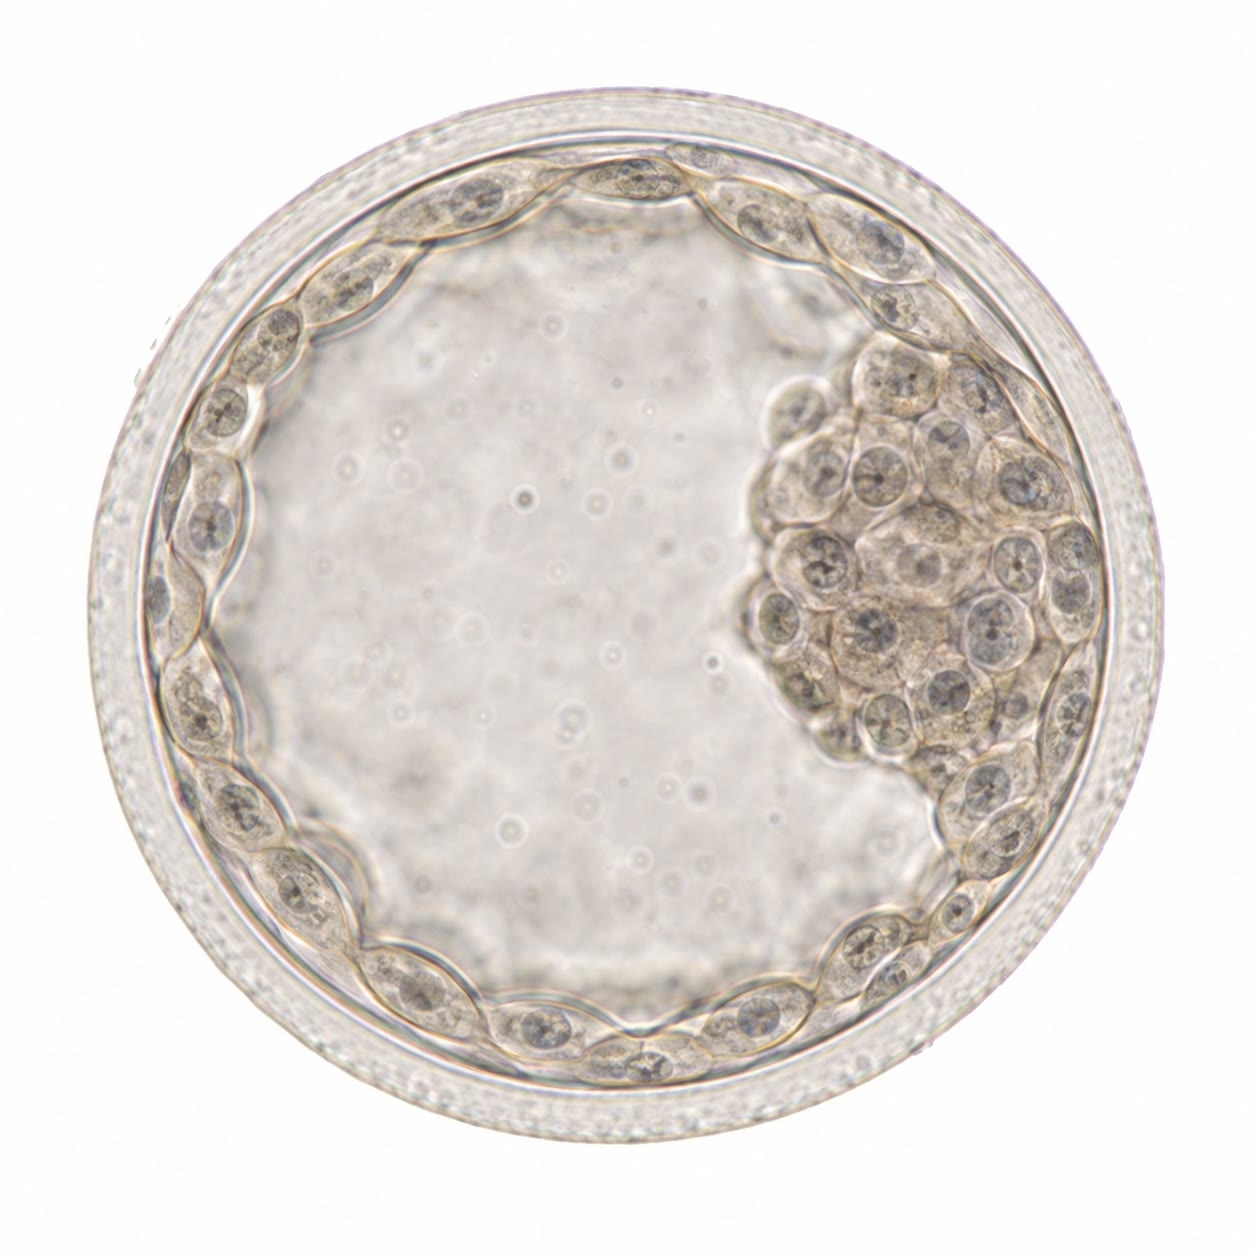
\includegraphics[width=0.42\linewidth]{images/book4/ai/b4-08-blastocyst.jpg}

{\small Um \omterm{def:b2:mammal-reproduction:implantation}{blastocisto} no quinto dia: o \omterm{def:b2:mammal-reproduction:implantation}{trofoblasto} externo em torno da
cavidade e a \omterm{def:b2:mammal-reproduction:implantation}{massa celular interna} --- o futuro embrião --- de um
lado.}
\end{omfigure}

\begin{definition}[A placenta]\label{def:b2:mammal-reproduction:placenta}
\index{placenta}\index{vilosidade coriônica}\index{cordão umbilical}
A \emph{placenta} é um órgão construído em conjunto pelo embrião (o
córion, a partir do \omterm{def:b2:mammal-reproduction:implantation}{trofoblasto}) e pela mãe (o revestimento uterino).
\emph{Vilosidades coriônicas} em forma de dedos, ramificadas numa
superfície de cerca de \qty{12}{m^2} no fim da gestação, pendem em
lagos de sangue materno trazido pelas artérias uterinas a meio litro
por minuto; dentro de cada vilosidade correm capilares fetais, ligados
ao feto pelas duas artérias e pela veia do \emph{cordão umbilical}. Os
dois sangues nunca se misturam: são separados pela parede da
vilosidade, alguns micrômetros de \omterm{def:b2:mammal-reproduction:implantation}{trofoblasto} e de endotélio capilar,
através da qual o oxigênio, o $\mathrm{CO_2}$, a água, a ureia e as
moléculas lipossolúveis se difundem, a glicose e os aminoácidos são
levados por transportadores, e os anticorpos maternos (IgG) são
transportados por receptores, dando ao recém-nascido seus primeiros
meses de imunidade. A placenta é também uma glândula: desde os
primeiros dias, o \omterm{def:b2:mammal-reproduction:implantation}{trofoblasto} secreta a \emph{gonadotrofina coriônica
humana} (hCG), que mantém o \omterm{def:b2:mammal-reproduction:ovary}{corpo lúteo} produzindo progesterona, e a
partir do terceiro mês a própria placenta produz a progesterona e os
estrógenos que mantêm a gestação (\cref{ch:b2:reproductive-hormones}). Ela é, na prática, um
pulmão, um intestino, um rim e uma glândula endócrina que cresce por
nove meses e é descartada no nascimento.
\end{definition}

\begin{omfigure}
\begin{tikzpicture}[every node/.style={font=\scriptsize}, >=stealth]
  % maternal blood space
  \fill[omThm!12] (0,0) rectangle (8,3.6);
  \node[omThm!80!black, align=center] at (1.1,2.6) {sangue materno\\(espaço\\interviloso)};
  % uterine wall at bottom
  \fill[omExo!30] (0,-0.6) rectangle (8,0); \node at (4,-0.3) {parede uterina (materna)};
  \draw[->, thick, omThm] (1.0,-0.6) -- (1.0,0.6); \node[omThm, anchor=west] at (1.05,0.3) {artéria espiralada};
  \draw[->, thick, omDef!60!black] (7.0,0.6) -- (7.0,-0.6); \node[omDef!60!black, anchor=east] at (6.95,0.3) {veia uterina};
  % chorionic plate at top
  \fill[omDef!20] (0,3.6) rectangle (8,4.4); \node at (4,4.0) {placa coriônica (fetal)};
  % villi hanging down
  \foreach \x in {2.6,4.2,5.8} {
    \draw[thick, fill=omDef!8] (\x-0.35,3.6) -- (\x-0.4,1.4) .. controls (\x-0.4,0.9) and (\x+0.4,0.9) .. (\x+0.4,1.4) -- (\x+0.35,3.6);
    \draw[thick, omThm!70!black] (\x-0.15,3.6) -- (\x-0.15,1.5) .. controls (\x-0.15,1.25) and (\x+0.15,1.25) .. (\x+0.15,1.5) -- (\x+0.15,3.6);
    \foreach \y in {2.0,2.7} { \draw[thick, fill=omDef!8] (\x-0.4,\y) .. controls (\x-0.9,\y+0.1) and (\x-0.9,\y-0.4) .. (\x-0.4,\y-0.3); }
  }
  % umbilical vessels
  \draw[very thick, omThm!70!black] (4.2,4.4) -- (4.2,5.0) node[above, align=center] {veia umbilical (para o feto)\\e artérias};
  \draw[very thick, omDef!60!black] (3.9,4.4) -- (3.9,5.0); \draw[very thick, omDef!60!black] (4.5,4.4) -- (4.5,5.0);
  % exchange arrows
  \draw[<->, thick] (3.0,2.2) -- (3.75,2.2); \node[anchor=west, align=left] at (8.3,1.5) {através da parede: \textcolor{omThm}{O$_2$, glicose,}\\\textcolor{omThm}{aminoácidos, IgG} para o feto;\\\textcolor{omDef!60!black}{CO$_2$, ureia} para a mãe};
  \node[anchor=west, align=left] at (8.3,3.0) {parede da vilosidade: trofoblasto\\+ endotélio capilar fetal,\\alguns micrômetros};
  \draw (6.2,2.5) -- (8.3,3.0);
\end{tikzpicture}

{\small A \omterm{def:b2:mammal-reproduction:placenta}{placenta}: as vilosidades fetais, com capilares fetais, pendem
num espaço cheio de sangue materno vindo das artérias espiraladas. Os
dois sangues fazem trocas através da parede da vilosidade e nunca se
misturam.}
\end{omfigure}

\begin{theorem}[As trocas através da placenta]\label{thm:b2:mammal-reproduction:fick}
\index{lei de Fick!placenta}
Um gás que atravessa uma membrana de área $A$ e espessura $d$ passa a
uma taxa $J = K\,A\,\Delta P/d$, em que $\Delta P$ é a diferença de sua
pressão parcial e $K$ a permeabilidade do tecido. Para o oxigênio no
tecido, $K \approx \qty{3e-8}{mL/(cm.min.mmHg)}$; com $A =
\qty{12}{m^2}$, $d = \qty{3.5}{\micro m}$ e $\Delta P =
\qty{20}{mmHg}$ (\qty{40}{mmHg} maternos no espaço interviloso contra
\qty{20}{mmHg} na artéria umbilical), a \omterm{def:b2:mammal-reproduction:placenta}{placenta} poderia transferir
cerca de \qty{200}{mL} de oxigênio por minuto, umas oito vezes os
\qty{25}{mL/min} que um feto a termo consome. A transferência de
oxigênio é, portanto, limitada não pela difusão, mas pelo fluxo
sanguíneo; o feto funciona a uma baixa pressão de oxigênio e compensa
com uma hemoglobina de maior afinidade e uma contagem maior de
hemácias.
\end{theorem}
\begin{proof}
A lei de Fick diz que o fluxo é proporcional ao gradiente
$\Delta P/d$ e à área; a constante $K$ incorpora a solubilidade e o
coeficiente de difusão do gás no tecido. Numericamente:
$3\times 10^{-8}\times 1.2\times 10^{5}\times 20/(3.5\times 10^{-4})
= \qty{206}{mL/min}$ com $A$ em \unit{cm^2} e $d$ em \unit{cm}. A
demanda fetal é de cerca de \qty{7}{mL} por quilograma por minuto para
\qty{3.5}{kg}.
\end{proof}

\section{Gestação, parto e lactação}

\begin{proposition}[Gestação e parto]\label{prop:b2:mammal-reproduction:birth}
\index{gestação}\index{parto}\index{ocitocina}
A gestação dura \num{20} dias no camundongo, \num{280} no ser humano e
\num{660} no elefante --- aproximadamente como a potência um quarto da
massa corporal, com os primatas lentos para o seu tamanho. Ela é
mantida pela progesterona, que mantém o músculo uterino em repouso e o
colo do útero fechado. O nascimento (\emph{parto}) é desencadeado pelo
próprio feto: o cortisol de suas suprarrenais, que sobe no fim da
gestação, faz a \omterm{def:b2:mammal-reproduction:placenta}{placenta} passar da progesterona ao estrógeno, que dota
o útero de receptores de ocitocina e de junções comunicantes e inicia
a liberação de prostaglandinas. Então uma \emph{retroalimentação
positiva} assume o controle: a cabeça pressiona o colo do útero,
nervos sensitivos sinalizam ao hipotálamo, a \emph{ocitocina} é
liberada pela neuro-hipófise, o útero se contrai, a cabeça pressiona
com mais força; a alça se intensifica até o nascimento, após o qual o
estímulo cessa e a alça para --- uma das poucas retroalimentações
positivas da fisiologia, e uma que precisa terminar num evento. A
\omterm{def:b2:mammal-reproduction:placenta}{placenta} é expelida minutos depois.
\end{proposition}
\begin{proof}[Evidências]
Ferguson (1941) mostrou no coelho que distender o colo do útero
provocava contrações uterinas e que seccionar a medula espinal ou
remover a neuro-hipófise abolia a resposta: um reflexo neuroendócrino
do colo à hipófise e ao útero. A ocitocina, isolada e sintetizada por
du Vigneaud em 1953, é hoje o fármaco padrão para induzir o trabalho
de parto.
\end{proof}

\begin{proposition}[A lactação]\label{prop:b2:mammal-reproduction:lactation}
\index{lactação}\index{prolactina}\index{leite}
A glândula mamária, uma glândula sudorípara modificada, é construída
durante a gestação pelo estrógeno, pela progesterona e pela prolactina,
mas impedida de secretar pela progesterona; quando a \omterm{def:b2:mammal-reproduction:placenta}{placenta} sai, a
progesterona cai e, sob a ação da \emph{prolactina} da adeno-hipófise,
os alvéolos começam a produzir leite. Dois reflexos comandam o
processo: a sucção estimula a liberação de prolactina (que mantém a
síntese e suprime a \omterm{def:b2:mammal-reproduction:ovary}{ovulação}) e a de ocitocina (que contrai as células
em torno dos alvéolos e ejeta o leite). O leite humano contém cerca de
\qty{7}{\%} de lactose, \qty{4}{\%} de gordura, \qty{1}{\%} de
proteína e \qty{2.9}{kJ/mL}; o \emph{colostro} dos primeiros dias é
rico em anticorpos (IgA) que revestem o intestino do bebê. Uma mãe
produz cerca de \qty{750}{mL} por dia, a um custo de cerca de
\qty{2.5}{MJ} --- um quarto de sua alimentação --- durante meses; a
lactação é a parte mais cara da reprodução dos mamíferos, e a que dá
nome à classe.
\end{proposition}

\section{A formação dos dois sexos}

\begin{proposition}[Determinação e diferenciação do sexo]\label{prop:b2:mammal-reproduction:sex}
\index{SRY}\index{hormônio anti-Mülleriano}\index{diferenciação sexual}
Até a sexta semana, um embrião humano de qualquer sexo tem o mesmo
equipamento: uma gônada indiferenciada, dois pares de ductos (de
\emph{Wolff} e de \emph{Müller}) e genitália externa neutra. O gene
\emph{SRY}, no cromossomo Y, é ativado na gônada e a transforma num
\omterm{def:b2:mammal-reproduction:testis}{testículo}; sem ele, a gônada se torna um ovário. O \omterm{def:b2:mammal-reproduction:testis}{testículo} fetal faz
então duas coisas: suas \omterm{def:b2:mammal-reproduction:testis}{células de Sertoli} secretam o \emph{\omterm{prop:b2:mammal-reproduction:sex}{hormônio
anti-Mülleriano}}, que faz os ductos de Müller regredirem, e suas
\omterm{def:b2:mammal-reproduction:testis}{células de Leydig} secretam \emph{testosterona}, que mantém os ductos de
Wolff (os futuros epidídimo, ducto deferente e vesículas seminais) e,
convertida em di-hidrotestosterona, molda a genitália externa em pênis
e escroto. Na ausência dos dois sinais, os ductos de Wolff regridem, os
ductos de Müller se tornam as tubas uterinas, o útero e a parte
superior da vagina, e a genitália se desenvolve como feminina. O
caminho feminino é o que se toma quando nada é dito: o caminho
masculino precisa ser imposto ativamente pelo \omterm{def:b2:mammal-reproduction:testis}{testículo}, e cada etapa
em que a imposição falha --- um SRY mutante, um receptor hormonal
ausente --- dá um indivíduo XY com corpo feminino ou intermediário.
\end{proposition}
\begin{proof}[Evidências]
Jost (1947) removeu as gônadas de fetos de coelho, ainda no útero,
antes que seus ductos se diferenciassem: os fetos castrados de ambos os
sexos cromossômicos desenvolveram útero, tubas uterinas e genitália
feminina. Um cristal de testosterona implantado num feto castrado
manteve os ductos de Wolff daquele lado, mas não eliminou os ductos de
Müller; um \omterm{def:b2:mammal-reproduction:testis}{testículo} fetal enxertado fez as duas coisas, do seu próprio
lado: o \omterm{def:b2:mammal-reproduction:testis}{testículo} precisa produzir um segundo fator, então
desconhecido, para suprimir os ductos femininos, identificado trinta
anos depois como o \omterm{prop:b2:mammal-reproduction:sex}{hormônio anti-Mülleriano}. Mais tarde, o efeito de
reversão sexual de um pequeno fragmento do cromossomo Y localizou o
interruptor no \emph{SRY} (1990), e um camundongo XX portador apenas do
gene \emph{Sry} se desenvolveu como macho.
\end{proof}

\begin{omfigure}
\begin{tikzpicture}[every node/.style={font=\scriptsize}, >=stealth]
  \node[draw, rounded corners, fill=omExo!25, align=center] (g) at (0,0) {gônada indiferenciada\\dois sistemas de ductos};
  \node[draw, rounded corners, fill=omDef!15, align=center] (t) at (4.2,1.4) {testículo\\(\emph{SRY} presente)};
  \node[draw, rounded corners, fill=omThm!15, align=center] (o) at (4.2,-1.4) {ovário\\(sem \emph{SRY})};
  \node[draw, rounded corners, fill=omDef!15, align=center] (amh) at (8.6,2.3) {AMH: os ductos de Müller regridem};
  \node[draw, rounded corners, fill=omDef!15, align=center] (tst) at (8.6,0.6) {testosterona: ductos de Wolff mantidos;\\DHT: genitália externa masculina};
  \node[draw, rounded corners, fill=omThm!15, align=center] (f) at (8.6,-1.4) {sem sinal: os ductos de Wolff regridem,\\ductos de Müller $\to$ tubas uterinas, útero;\\genitália feminina};
  \draw[->, thick] (g) -- (t); \draw[->, thick] (g) -- (o);
  \draw[->, thick] (t) -- (amh); \draw[->, thick] (t) -- (tst); \draw[->, thick] (o) -- (f);
\end{tikzpicture}

{\small A \omterm{prop:b2:mammal-reproduction:sex}{diferenciação sexual}: o \omterm{def:b2:mammal-reproduction:testis}{testículo}, formado sob a ação do
\emph{SRY}, impõe o caminho masculino com dois hormônios; na ausência
deles, o corpo se desenvolve como feminino.}
\end{omfigure}

\section{Exercícios}

\begin{exercise}[$\star$]\label{exo:b2:mammal-reproduction:1}
Compare a \omterm{def:b2:mammal-reproduction:testis}{espermatogênese} e a \omterm{def:b2:mammal-reproduction:ovary}{ovogênese}: quando as células-tronco se
dividem, quantos gametas uma \omterm{def:b2:meiosis-heredity:meiosis}{meiose} produz, quanto tempo leva a
produção de um gameta, onde ficam as paradas e quantos gametas são
produzidos ao longo da vida.
\end{exercise}

\begin{exercise}[$\star$]\label{exo:b2:mammal-reproduction:2}
Liste as etapas da fecundação, desde a chegada de um espermatozoide à
zona até a primeira mitose, e diga qual etapa bloqueia a polispermia.
\end{exercise}

\begin{exercise}[$\star$]\label{exo:b2:mammal-reproduction:3}
Cite as duas populações celulares do \omterm{def:b2:mammal-reproduction:implantation}{blastocisto} e o destino de cada
uma. Em que dia começa a \omterm{def:b2:mammal-reproduction:implantation}{implantação}, e que hormônio precisa ter
preparado o útero?
\end{exercise}

\begin{exercise}[$\star$]\label{exo:b2:mammal-reproduction:4}
Para cada item a seguir, diga se atravessa a \omterm{def:b2:mammal-reproduction:placenta}{placenta} e como: oxigênio,
glicose, hemácias maternas, anticorpos IgG, ureia, álcool, a maioria
das bactérias.
\end{exercise}

\begin{exercise}[$\star\star$]\label{exo:b2:mammal-reproduction:5}
Com $\pi = 10^{-8}$ por espermatozoide, calcule a probabilidade de
fecundação para contagens de espermatozoides de $3\times 10^{8}$,
$10^{8}$, $4\times 10^{7}$ e $10^{7}$. Em que contagem ela cai abaixo
de metade? O que isso diz sobre a forma da relação dose--resposta
entre a fertilidade e a contagem de espermatozoides?
\end{exercise}

\begin{exercise}[$\star\star$]\label{exo:b2:mammal-reproduction:6}
Uma menina nasce com $10^{6}$ ovócitos, tem \num{300000} na puberdade
(aos 13 anos) e cerca de \num{1000} aos 50, tendo ovulado \num{400}.
Calcule a taxa média de atresia (ovócitos perdidos por dia) antes e
depois da puberdade, e compare com a taxa de \omterm{def:b2:mammal-reproduction:ovary}{ovulação}.
\end{exercise}

\begin{exercise}[$\star\star$]\label{exo:b2:mammal-reproduction:7}
A hemoglobina fetal tem uma pressão de meia saturação $P_{50} =
\qty{19}{mmHg}$, e a hemoglobina adulta, \qty{27}{mmHg}; tome a
saturação como $S = P^{n}/(P_{50}^{n} + P^{n})$ com $n = 2.7$. Calcule
as duas saturações a \qty{30}{mmHg}, a pressão na veia umbilical, e
explique a vantagem.
\end{exercise}

\begin{exercise}[$\star\star$]\label{exo:b2:mammal-reproduction:8}
A hCG aparece no sangue materno na \omterm{def:b2:mammal-reproduction:implantation}{implantação} (dia 7 após a
fecundação) a cerca de \qty{1}{UI/L} e dobra a cada dois dias; um teste
de gravidez detecta \qty{25}{UI/L}. Em que dia após a fecundação o
teste dá positivo? Em que dia após a última menstruação (com \omterm{def:b2:mammal-reproduction:ovary}{ovulação}
no dia 14)?
\end{exercise}

\begin{exercise}[$\star\star$]\label{exo:b2:mammal-reproduction:9}
Recalcule a transferência placentária de oxigênio do teorema para uma
\omterm{def:b2:mammal-reproduction:placenta}{placenta} de \qty{6}{m^2} com uma parede de vilosidade de
\qty{10}{\micro m}, como em algumas patologias, e compare com a demanda
fetal. O que acontece com o feto?
\end{exercise}

\begin{exercise}[$\star\star\star$]\label{exo:b2:mammal-reproduction:10}
Preveja o sistema de ductos e a genitália externa de: (a) um feto XY
cujas células não têm o receptor de testosterona; (b) um feto XY sem
\omterm{prop:b2:mammal-reproduction:sex}{hormônio anti-Mülleriano}; (c) um feto XX exposto a muita testosterona
vinda de suas suprarrenais; (d) um feto XX que leva o \emph{SRY} num
cromossomo X. Explique cada caso a partir dos resultados de Jost.
\end{exercise}

\begin{exercise}[$\star\star\star$]\label{exo:b2:mammal-reproduction:11}
Os gêmeos idênticos surgem quando um embrião se divide. Se ele se
divide antes do dia 3, os gêmeos têm \omterm{def:b2:mammal-reproduction:placenta}{placentas} e bolsas separadas;
entre os dias 4 e 8, uma \omterm{def:b2:mammal-reproduction:placenta}{placenta} e duas bolsas; entre os dias 8 e 13,
uma \omterm{def:b2:mammal-reproduction:placenta}{placenta} e uma bolsa; mais tarde, são siameses. Numa série de
gêmeos idênticos, \qty{30}{\%} têm \omterm{def:b2:mammal-reproduction:placenta}{placentas} separadas, \qty{68}{\%}
uma \omterm{def:b2:mammal-reproduction:placenta}{placenta} e duas bolsas, \qty{2}{\%} uma bolsa. Deduza que estágio
do desenvolvimento se divide com mais frequência, e explique em
termos do \omterm{def:b2:mammal-reproduction:implantation}{blastocisto} quais estruturas são compartilhadas em cada caso.
\end{exercise}

\begin{exercise}[$\star\star\star$]\label{exo:b2:mammal-reproduction:12}
Os marsupiais dão à luz, após poucas semanas, um filhote do tamanho de
um feijão, que completa seu crescimento preso a uma teta na bolsa; os
mamíferos placentários têm gestações longas e dão à luz um filhote
grande. Compare as duas estratégias em termos de custo materno, de
risco e da capacidade da mãe de abandonar uma ninhada numa estação
ruim, e sugira por que os placentários deslocaram os marsupiais em
todos os continentes, exceto a Austrália.
\end{exercise}

\section{Problema: Uma gravidez em números}

\begin{problem}[{Problema de fim de semana --- uma gravidez humana
acompanhada do espermatozoide ao leite, pelas probabilidades de
fecundação, pelo calendário da implantação e de seu hormônio, pela
capacidade de trocas da placenta e pelo custo energético da gestação e
da lactação, até a probabilidade de fecundação, o dia em que o teste
dá positivo, a margem de oxigênio da placenta e o custo de um dia de
leite}]
\label{pb:b2:mammal-reproduction:1}
Dados: $3\times 10^{8}$ espermatozoides por ejaculação, cada um
alcançando o óvulo com probabilidade $10^{-8}$; os espermatozoides
nadam a \qty{50}{\micro m/s}; a ampola fica a \qty{15}{cm} do colo do
útero. hCG na \omterm{def:b2:mammal-reproduction:implantation}{implantação} (dia 7) de
\qty{1}{UI/L}, dobrando a cada \qty{2}{d}, limiar do teste de
\qty{25}{UI/L}. \omterm{def:b2:mammal-reproduction:placenta}{Placenta} a termo: \qty{12}{m^2}, parede de
\qty{3.5}{\micro m}, $K_{\mathrm{O_2}} = \qty{3e-8}{mL/(cm.min.mmHg)}$,
$\Delta P = \qty{20}{mmHg}$; feto de \qty{3.5}{kg} que consome
\qty{7}{mL} de oxigênio por quilograma por minuto; fluxo sanguíneo
placentário materno de \qty{500}{mL/min}, com \qty{0.16}{mL} de
oxigênio por mililitro de sangue. Glicose: o feto usa \qty{5}{mg} por
quilograma por minuto; sangue materno a \qty{0.9}{g/L}. Leite:
\qty{750}{mL/d} a \qty{2.9}{kJ/mL}, produzido com \qty{80}{\%} de
eficiência; o bebê ganha \qty{30}{g/d} de tecido a \qty{6}{kJ/g}
depositados e gasta \qty{300}{kJ/kg/d} com a manutenção, pesando
\qty{4}{kg}.

\medskip
\noindent\textbf{Parte I --- A fecundação.}
\begin{enumerate}
  \item Calcule o número médio de espermatozoides que alcançam o óvulo
        e a probabilidade de fecundação.
  \item Calcule a probabilidade de que dois ou mais o alcancem, e diga
        o que aconteceria sem a \omterm{prop:b2:mammal-reproduction:fertilisation}{reação cortical}.
  \item Quanto tempo um espermatozoide levaria para nadar até a ampola?
        Espermatozoides são encontrados ali em \qty{30}{min}: o que os
        leva?
  \item Só algumas centenas de espermatozoides chegam à ampola. Que
        fração da ejaculação é essa, e onde os outros se perdem?
  \item Um óvulo pode ser fecundado durante cerca de um dia, e os
        espermatozoides sobrevivem cerca de três dias no trato. Durante
        quantos dias do ciclo uma relação sexual pode levar à
        concepção?
  \item A contagem de um homem cai para $5\times 10^{7}$. Recalcule a
        probabilidade de fecundação por ciclo e o número esperado de
        ciclos até a concepção (lei geométrica).
  \item Explique por que é o óvulo, e não o espermatozoide, que fornece
        as mitocôndrias do embrião.
\end{enumerate}

\medskip
\noindent\textbf{Parte II --- A \omterm{def:b2:mammal-reproduction:implantation}{implantação} e seu hormônio.}
\begin{enumerate}[resume]
  \item Quantas divisões de clivagem ocorreram até o dia 5, se cada uma
        leva \qty{16}{h}? Quantas células?
  \item Em que dia após a fecundação a hCG atinge o limiar do teste? E
        após a última menstruação (\omterm{def:b2:mammal-reproduction:ovary}{ovulação} no dia 14)?
  \item Por que a hCG precisa aparecer poucos dias após a \omterm{def:b2:mammal-reproduction:implantation}{implantação}?
        O que acontece com o \omterm{def:b2:mammal-reproduction:ovary}{corpo lúteo}, e com a gestação, se ela não
        aparecer?
  \item A hCG atinge um pico perto de \qty{1e5}{UI/L} por volta da
        semana 10 e depois cai. Quantas duplicações desde a \omterm{def:b2:mammal-reproduction:implantation}{implantação}
        isso representa, e por que ela pode cair depois sem perda da
        gestação?
  \item Metade das concepções se perde antes da \omterm{def:b2:mammal-reproduction:implantation}{implantação} ou nela,
        sobretudo por óvulos aneuploides. Explique por que a
        aneuploidia é mais comum nos óvulos que nos espermatozoides,
        usando o calendário da \omterm{def:b2:mammal-reproduction:ovary}{ovogênese}.
  \item Gêmeos: um embrião que se divide no dia 6. Diga se os gêmeos
        compartilham a \omterm{def:b2:mammal-reproduction:placenta}{placenta} e a bolsa amniótica.
\end{enumerate}

\medskip
\noindent\textbf{Parte III --- A \omterm{def:b2:mammal-reproduction:placenta}{placenta}.}
\begin{enumerate}[resume]
  \item Calcule a transferência difusiva máxima de oxigênio.
  \item Calcule a demanda fetal de oxigênio e a margem de difusão.
  \item Calcule o oxigênio entregue por minuto à \omterm{def:b2:mammal-reproduction:placenta}{placenta} pelo fluxo
        sanguíneo materno. Que fração precisa ser extraída para atender
        à demanda?
  \item Calcule a demanda fetal de glicose em gramas por dia e o volume
        de sangue materno que a contém. Compare com o fluxo placentário
        materno diário.
  \item O sangue do feto sai da \omterm{def:b2:mammal-reproduction:placenta}{placenta} a \qty{30}{mmHg} de oxigênio.
        Por que ele não sufoca a uma pressão que deixaria um adulto
        inconsciente?
  \item Cite duas coisas que a \omterm{def:b2:mammal-reproduction:placenta}{placenta} faz e que nenhum outro órgão do
        embrião poderia fazer nessa época, e uma coisa que ela não
        consegue fazer.
\end{enumerate}

\medskip
\noindent\textbf{Parte IV --- O parto e o leite.}
\begin{enumerate}[resume]
  \item Descreva a retroalimentação positiva do trabalho de parto e
        explique por que ela não dispara antes do termo.
  \item Calcule a energia do leite de um dia e a energia que a mãe gasta
        para produzi-lo.
  \item Calcule o balanço energético diário do bebê (crescimento mais
        manutenção) e compare com o leite fornecido.
  \item Calcule o custo energético total de nove meses de lactação para
        a mãe, e compare com o custo de \qty{300}{MJ} da própria
        gestação.
  \item Explique por que a sucção retarda o retorno da \omterm{def:b2:mammal-reproduction:ovary}{ovulação}, e por
        que isso importa em populações sem contracepção.
  \item Enuncie o resultado: a probabilidade de fecundação, o dia em
        que o teste dá positivo, a margem de oxigênio da \omterm{def:b2:mammal-reproduction:placenta}{placenta} e o
        custo de um dia de leite.
\end{enumerate}
\end{problem}
